\documentclass{article} % For LaTeX2e
\usepackage{nips15submit_e,times}
\usepackage{hyperref}
\usepackage{url}
\usepackage{graphicx}
\usepackage{amsfonts}
\usepackage{amsmath}
%\documentstyle[nips14submit_09,times,art10]{article} % For LaTeX 2.09


\title{Handwritten Digits Classification using Logistic and Softmax Regression}


\author{
Sriram Ravindran\\
Department of Computer Science\\
A53208651 \\
\texttt{sriram@ucsd.edu} \\
\And
Ojas Gupta \\
A53201624 \\
\texttt{ogupta@ucsd.edu} \\
}

% The \author macro works with any number of authors. There are two commands
% used to separate the names and addresses of multiple authors: \And and \AND.
%
% Using \And between authors leaves it to \LaTeX{} to determine where to break
% the lines. Using \AND forces a linebreak at that point. So, if \LaTeX{}
% puts 3 of 4 authors names on the first line, and the last on the second
% line, try using \AND instead of \And before the third author name.

\newcommand{\fix}{\marginpar{FIX}}
\newcommand{\new}{\marginpar{NEW}}

%\nipsfinalcopy % Uncomment for camera-ready version

\begin{document}


\maketitle
\begin{abstract}
Here in this project we have implemented the famous Logistic Regression which is a two class classifier and its extension Softmax Regression which is a multiclass classifier. Both of these methods are trained and tested on famous handwritten MNIST dataset via gradient descent. We used the first 20000 data points as our training set out of which we have kept the 10 percent i.e. 2000 as our hold out set. On training our system we have tested on the first 2000 test data points so as to evaluate our work. On using the Logistic Regression, we have attained an accuracy of " " while classifying 2 vs 3 and an accuracy " " while classifying 2 vs 8. On applying 10 way classification, we get an accuracy of " ". To enhance classification and generalization we have used regularization as well. 
\end{abstract}

\section{Keywords}
%% Your NIPS paper can be submitted with any of the following keywords (more than one keyword is possible for each paper):

\begin{verbatim}
Neural Networks, Logistic Regression, Softmax Regression
\end{verbatim}
\section{Derivation of Gradient for Logistic Regression}
We will derive the gradient for logistic regression by using the following predefined variables given in the document.

Given:
\begin{center}
	$y^n=\cfrac{1}{1+exp(-w^T x^n)}$(Sigmoid function)\\
    \hfill\break
    $E(w) = -\sum_N t^n lny^n + (1-t^n) ln(1-y^n)$\\
    \hfill\break
\end{center}
To Prove:
\begin{center}
    -$\cfrac{\partial E^n(w)}{\partial w_j} = (t^n-y^n)x^n_j $\\
    \hfill\break
\end{center}
\begin{center}
Let's recall the properties of Sigmoid Function, if $\sigma(x)$ is a sigmoid function then following two properties hold:\\
\hfill\break
1) $\sigma(x)=1-\sigma(-x)$\\
\hfill\break
2) $\sigma'(x)=\sigma(x)\sigma(-x)$\\
\hfill\break
\end{center}
Derivation:
\begin{center}
$E^n(w) = -(t^n lny^n + (1-t^n) ln(1-y^n))$\\
\hfill\break
\hfill\break
$\cfrac{\partial E^n(w)}{\partial w_j} = -(\cfrac{t^n}{y^n} - \cfrac{1-t^n}{1-y^n})\cfrac{\partial y^n}{\partial w_j}$\\
    \hfill\break
    \hfill\break
$\cfrac{\partial E^n(w)}{\partial w_j} = -(\cfrac{t^n-y^n}{y^n(1-y^n)})\cfrac{\partial y^n}{\partial w_j}$\\
    \hfill\break
    \hfill\break
$\cfrac{\partial E^n(w)}{\partial w_j} = -(\cfrac{t^n-y^n}{y^n(1-y^n)})y^n(1-y^n)\cfrac{\partial w^Tx}{\partial w_j}$(Properties of Sigmoid)\\
    \hfill\break
    \hfill\break
$\cfrac{\partial E^n(w)}{\partial w_j} = -(t^n-y^n)\cfrac{\partial w^Tx^n}{\partial w_j}$\\
    \hfill\break
    \hfill\break
$\cfrac{\partial E^n(w)}{\partial w_j} = -(t^n-y^n)x^n_j$\\
    \hfill\break
    Hence Proved 

\end{center}
\section{Derivation of Gradient for Softmax Regression}
We will derive the gradient for softmax regression by using the following predefined variables given in the document.

Given:
\begin{center}
	$y_k^n = \cfrac{exp(a_{k}^n)}{\sum_k' exp(a_k'^n)}$\\
    \hfill\break
$a_{k}^n = w_k^T x^n$\\
\hfill\break
$E = −\sum_n \sum_{k=1}^{c} t^n_k ln(y_k^n)$
\end{center}
To Prove:
\begin{center}
    -$\cfrac{\partial E^n(w)}{\partial w_j^k} = (t^n_k-y^n_k)x^n_j $\\
    \hfill\break
\end{center}
Derivation:
\begin{center}
$E^n(w) = -\sum_{k'=1}^{c} t^n_{k'} ln(y_{k'}^n)$\\
\hfill\break
\hfill\break
$\cfrac{\partial E^n(w)}{\partial w_{jk}} = -\sum_{k'=1}^{c}\cfrac{\partial(t^n_{k'}ln(exp(w_{k'}^Tx^n))-t^n_{k'}ln(\sum_{k''}exp(w_{k''}^Tx^n)))}{\partial w_{jk}}$\\
	\hfill\break
    \hfill\break
$\cfrac{\partial E^n(w)}{\partial w_{jk}} = -\sum_{k'=1}^{c}\cfrac{\partial(t^n_{k'}w_{k'}^Tx^n-t^n_{k'}ln(\sum_{k''}exp(w_{k''}^Tx^n)))}{\partial w_{jk}}$\\
    \hfill\break
    \hfill\break
$\cfrac{\partial E^n(w)}{\partial w_{jk}} = -t^n_kx^n_j-\sum_{k'=1}^{c}\cfrac{\partial (t^n_{k'}ln(\sum_{k''}exp(w_{k''}^Tx^n)))}{\partial w_{jk}}$\\
    \hfill\break
    \hfill\break
$\cfrac{\partial E^n(w)}{\partial w_{jk}} = -t^n_kx^n_j-\cfrac{\partial (ln(\sum_{k''}exp(w_{k''}^Tx^n)))}{\partial w_{jk}}$\\
    \hfill\break
    \hfill\break
$\cfrac{\partial E^n(w)}{\partial w_{jk}} = -t^n_kx^n_j-\cfrac{exp(w_k^Tx^n)}{\sum_{k''}exp(w_{k''}^Tx^n))}x^n_j$\\
    \hfill\break
    \hfill\break
$\cfrac{\partial E^n(w)}{\partial w_{jk}} = -t^n_kx^n_j-y_k^nx^n_j$\\
    \hfill\break
    \hfill\break
$\cfrac{\partial E^n(w)}{\partial w_{jk}} = -(t^n_k-y_k^n)x^n_j$\\
    \hfill\break
    Hence Proved 

\end{center}

\section{Logistic Regression}
Although we consider logistic regression to be a classification technique, it is called "regression" because it is used to fit a continuous variable: the probability of the category, given the data. Logistic regression can be modeled as using a single neuron reading in an input vector (1,{\sl x}) $\in \mathbb{R}^{d+1}$ and parameterized by weight vector {\sl w} $\in \mathbb{R}^{d+1}$ . d is the dimensionality of the input, and we tack on a "1" at the beginning for a bias parameter, $w_0$ . The neuron outputs the probability that x is a member of class $C_1$.\\
\begin{center}
P $(x \in C_1 |x) = \frac{1}{1+exp(-w^T x)}$\\
P $(x \in C_2 |x)$ = 1 − P$(x \in C_1 |x)$
\end{center}
where g w (x) simply notes that the function g is parameterized by w. Note we identify the output y n of the "network"
for a particular example, x n , with g w (x n ), i.e., y n = g w (x n ). With the hypothesis function defined, we now use
the cross entropy loss function (Equation 3) for two categories over our training examples. This equation measures
how well our hypothesis function g does over the N data points,
E(w) = −
N
X
{t n ln y n + (1 − t n ) ln(1 − y n )}.
(3)
n=1
Here, t n is the target or teaching signal for example n. Our goal is to optimize this cost function via gradient
descent. This cost function is minimized at 0 when t n = y n for all n. One issue with this cost function is that it
depends on the number of training examples. For reporting purposes in this assignment, a more convenient measure
is the average error:
E(w) = −
N
1 X n
{t ln y n + (1 − t n ) ln(1 − y n )}.
\subsection{Introduction}
Using the gradient derived for Logistic Regression cross entropy loss, we will first use gradient descent to classify for categories: 2's and 3's, 2's and 8's.  

Now, using the gradient derived for Logistic Regression cross entropy loss, use gradient descent to classify x ∈ R 785 (there is one extra dimension for the bias term) for two categories: 2’s and 3’s. The target is 1 if the input is from the "2" category and 0 if it is from the other category. 
\subsection{Method}
\subsection{Results and Discussion}

We have calculated the entropy and classification accuracy of 2 vs 3 and 2 vs 8 data set and the results are found to be quite impressive. Following are the graphs plotted for them. Figure 1 and 2 shows the entropy and classification accuracy of 2 vs 3

\begin{figure}[h]
\begin{center}
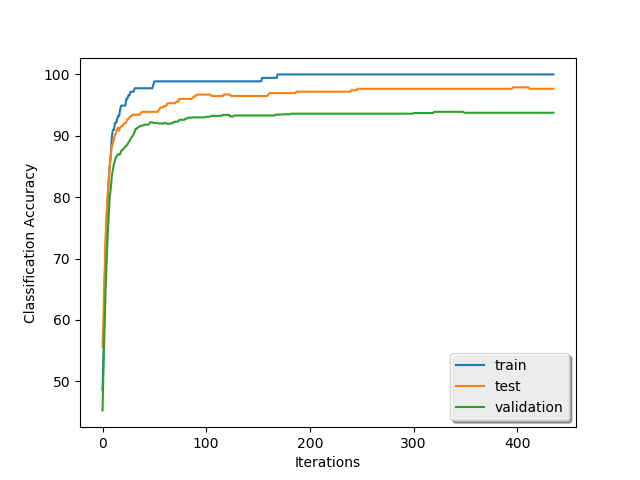
\includegraphics[width=0.8\linewidth]{plt_2vs3_accuracy.png}
\end{center}
\caption{Plot of accuracy in 2 vs 3.}
\end{figure}

\begin{figure}[h]
\begin{center}
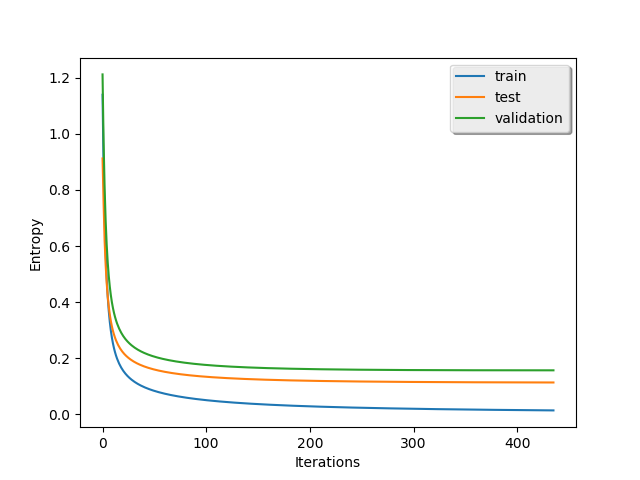
\includegraphics[width=0.8\linewidth]{plt_2vs3_losses.png}
\end{center}
\caption{Plot of entropy in 2 vs 3.}
\end{figure}

\begin{figure}[h]
\begin{center}
%\framebox[4.0in]{$\;$}
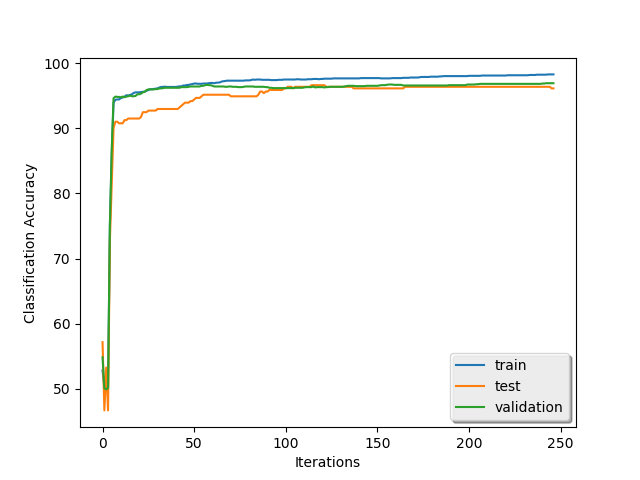
\includegraphics[width=0.8\linewidth]{plt_2vs8_accuracy.png}
\end{center}
\caption{Plot of accuracy in 2 vs 8.}
\end{figure}

\begin{figure}[h]
\begin{center}
%\framebox[4.0in]{$\;$}
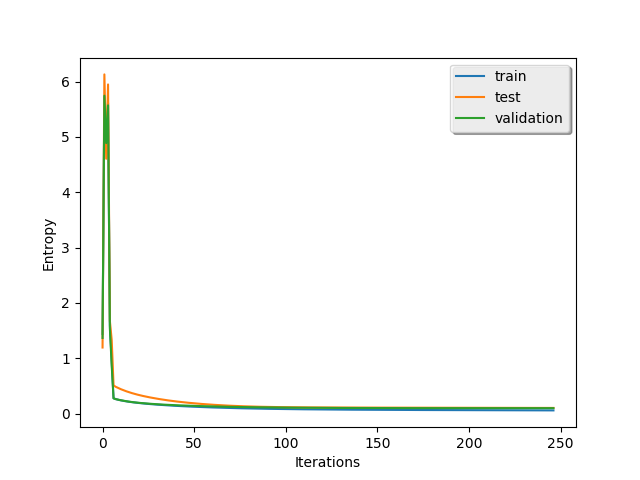
\includegraphics[width=0.8\linewidth]{plt_2vs8_losses.png}
\end{center}
\caption{Plot of losses in 2 vs 8.}
\end{figure}

\begin{figure}[h]
\begin{center}
%\framebox[4.0in]{$\;$}
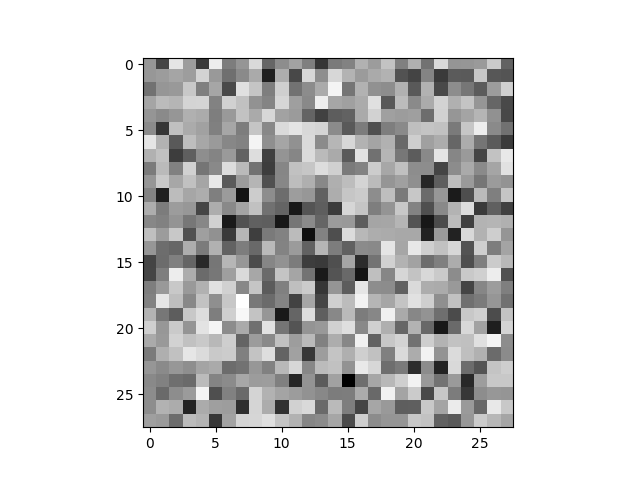
\includegraphics[width=0.8\linewidth]{2vs3-2vs8.png}
\end{center}
\caption{Sample figure caption.}
\end{figure}

\begin{figure}[h]
\begin{center}
%\framebox[4.0in]{$\;$}
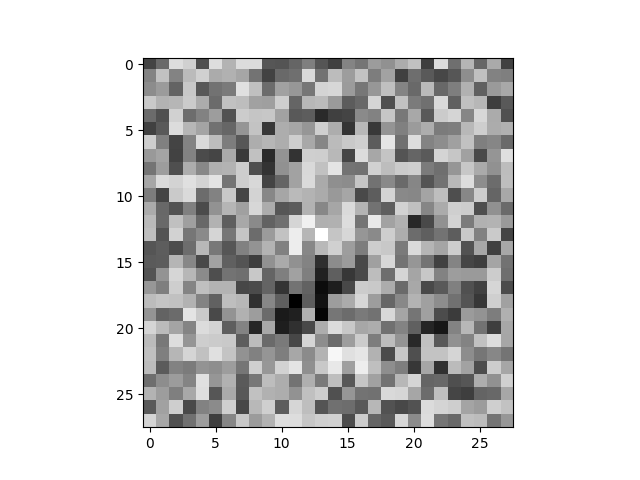
\includegraphics[width=\linewidth]{2vs3.png}
\end{center}
\caption{Sample figure caption.}
\end{figure}

\begin{figure}[h]
\begin{center}
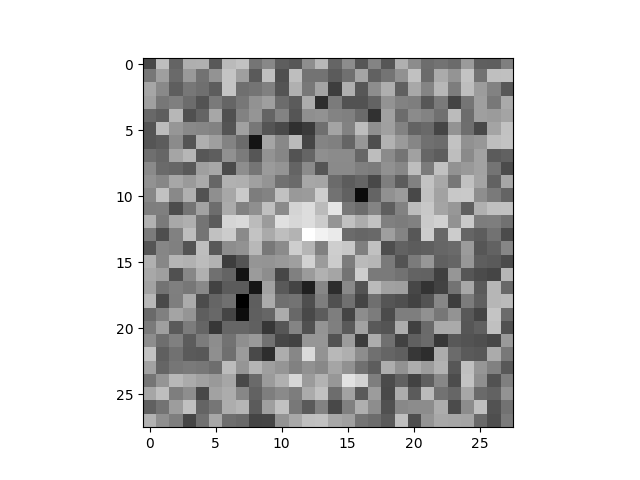
\includegraphics[width=\linewidth]{2vs8.png}
\end{center}
\caption{Sample figure caption.}
\end{figure}

\section{Softmax Regression}
Softmax regression is the generalization of logistic regression for multiple (c) classes. Now given an input $x^n$ , softmax regression will output a vector $y^n$ , where each element, $y_k^n$ represents the probability that $x^n$ is in class k.\\
\begin{center}
$y_k^n = \frac{exp(a_{k}^n)}{\sum_k' exp(a_k'^n)}$\\
$a_{k}^n = w_k^T x^n$\\
\end{center}

Here, $a_{k}^n$ is called the net input to output unit $y_k$. Note each output has its own weight vector $w_k$ . With our model defined, we now define the cross-entropy cost function for multiple categories:
\begin{center}
$E = −\sum_n \sum_{k=1}^{c} t^n_k ln(y_k^n)$
\end{center}

Again, taking the average of this over the number of training examples normalizes this error over different training set sizes.

Further information is distributed as section 3.1 contains the introduction to the problem, section 3.2 contains method used to solve the problem. Results ans Discussion is done in section 3.3 and 3.4 respectively.\\ 
\subsection{Introduction}
In this part of the problem, we have created a multi-class classifier which classifies a data point into 10 different classes. 
\subsection{Method}
\subsection{Results and Discussion}

\subsection{Tables}

All tables must be centered, neat, clean and legible. Do not use hand-drawn
tables. The table number and title always appear before the table. See
Table~\ref{sample-table}.

Place one line space before the table title, one line space after the table
title, and one line space after the table. The table title must be lower case
(except for first word and proper nouns); tables are numbered consecutively.

\begin{table}[t]
\caption{Sample table title}
\label{sample-table}
\begin{center}
\begin{tabular}{ll}
\multicolumn{1}{c}{\bf PART}  &\multicolumn{1}{c}{\bf DESCRIPTION}
\\ \hline \\
Dendrite         &Input terminal \\
Axon             &Output terminal \\
Soma             &Cell body (contains cell nucleus) \\
\end{tabular}
\end{center}
\end{table}

\end{document}
